% !TEX encoding = UTF-8 Unicode

\documentclass[a4paper]{article}

\usepackage{color}
\usepackage{url}
\usepackage[T2A]{fontenc} 
\usepackage[utf8]{inputenc}
\usepackage{graphicx}

\usepackage[english,serbian]{babel}
\usepackage[unicode]{hyperref}
\hypersetup{colorlinks,citecolor=red,filecolor=green,linkcolor=blue,urlcolor=blue}

\begin{document}

\title{Etika video igara\\ \small{Seminarski rad u okviru kursa\\Računarstvo i društvo\\ Matematički fakultet}}

\author{Slobodan Jovanović\\ mi17186@alas.matf.bg.ac.rs}
\date{1.~septembar 2022.}
\maketitle

\abstract{
Rad se bavi etikom u video igrama. Objašnjava zašto postavljamo etička pitanja kod video igara, kakav uticaj video igre imaju na društvo i primere tog uticaja. 
}
\tableofcontents

\newpage

\section{Uticaj video igara}
\label{sec:uvod}
Široka upotreba video igara u obrazovanju, obuci, zabavi i upotreba tehnologija
video igara u dizajnu i kontroli medicinskih, komercijalnih i vojnih sistema ima
značajan uticaj na sadašnje i buduće pravce društva.

Video igre postavljaju etička pitanja jer se u ovim igrama može, a ponekad ste i
podstaknuti na vršenje radnji koje su moralno zabranjene u stvarnom svetu. Mnogi
istraživači su ispitali moguće posledice podsticanja takvih akcija u stvarnom svetu
dok se drugi fokusiraju na pozitivne aspekte video igara u obrazovanju i obuci. Oba
pristupa se slažu u jednoj stvari, naime, da su ove igre u stanju da promene naše ideje o
svetu i kako se u njemu ponašamo.

Nema sumnje da video igre imaju značajan uticaj. Ponekad je uticaj pozitivan i koristan.
Koriste se u zdravstvu i obrazovanju. Koriste se da pomognu pacijentima da se rehabilituju od
operacije i povrede. Zbog svoje sposobnosti da poboljšaju koordinaciju ruku i očiju
koristi se u raznim sektorima od obuke letenja i hirurgije do vojne obuke. One se takođe
koriste za poboljšanje kritičkog mišljenja, kreativnosti i podsticanje istraživačkog pristupa
rešavanja problema. Napredna tehnologija video igara omugućava razvoj obrazovnih igara gde
igrači mogu da proučavaju istorijske događaje ponavljajući istoriju i da
oblikuju događaje svojim odlukama. U igrama kao što su {\em Sim City} igrači mogu simulirati društvo, u kome igraju neku
ulogu i da ispitaju ishode svojih postupaka. Pored ovih funkcija, obaveštajna agencija Sjedinjenih Američkih Država
koristi video igre za obuku svojih špijuna i vojnika. Ove igre nisu nasumične igre rata, 
one postavljaju agente u specifične situacije gde je cilj da ih nauče kako da
razmišljaju pod pritiskom, kako da rasuđuju i koriste nasilje samo kao krajnje sredstvo.
\newpage

\section{Šta čini ove igre toliko efikasnim u uticaju na pojedinca}
\label{sec:efikasno}
Postoje brojne studije o efikasnosti video igara i postoje razne
vrste video igara, od učenja ponavljanja jednostavnih sekvenci do igara koje od vas zahtevaju da donosite složene odluke u 3-d simulacijama. 
One zahtevaju aktivno učešće pojedinca, a za to je potrebno da se on usredsredi i posveti dosta pažnje. 
Učestvovanje pojedinca u video igri podrazumeva šablone koji se ponavljaju i nagrade za uspeh u igri. To su ključni
faktori u učenju i mogu uticati dosta na pojedinca. Težnja igrača je da u igri pobedi. Želja za tim može postati toliko velika, da će on učiti kako to da uradi.

Uticaj ovih igara je ilustrovan ovim primerom. Jednog groznog popodneva u
Iraku, dok se borio protiv pobunjenika u severnom gradu Mosulu, narednik je zapucao ka neprijatelju.
„Osećao sam se kao da sam u velikoj video igrici. Nije me čak ni uznemirilo, uzvratio sam.
Bio je prirodni instinkt. Bum! Bum! Bum! Bum!" priseća se narednik. Glavni
Oficir za modeliranje i simulaciju odbrane za vojsku je rekao. -: Kad je došlo vreme za njega
da ispali iz svog oružja, bio je spreman i sposoban da to uradi.
Njegovo iskustvo koje je vodilo do tog vremena, kroz treninge na terenu i igranje {\em Halo} i
drugih igara, omogućilo mu da je da uradi to. Njegova svest o situaciji je bila podignuta. Znao je šta treba da
uradi. On je to radio ranije, ili nešto slično pre toga.\cite{washingtonpost}

Nažalost, ova moć može i da se zloupotrebi za suptilnu manipulaciju mišljenja. {\em America's Army} je prva video igra koja je za cilj
imala regrutovanje u vojsku i prva igra koja je imala političke ciljeve. Kritičari su naveli da igra služi za širenje propagande. Kao i svaki uređaj koji se može koristiti u treningu, video igre se mogu koristiti za oblikovanje
ideja na pozitivan ili negativan način.\cite{wikipedia_american_army}

\begin{figure}[h!]
	\begin{center}
		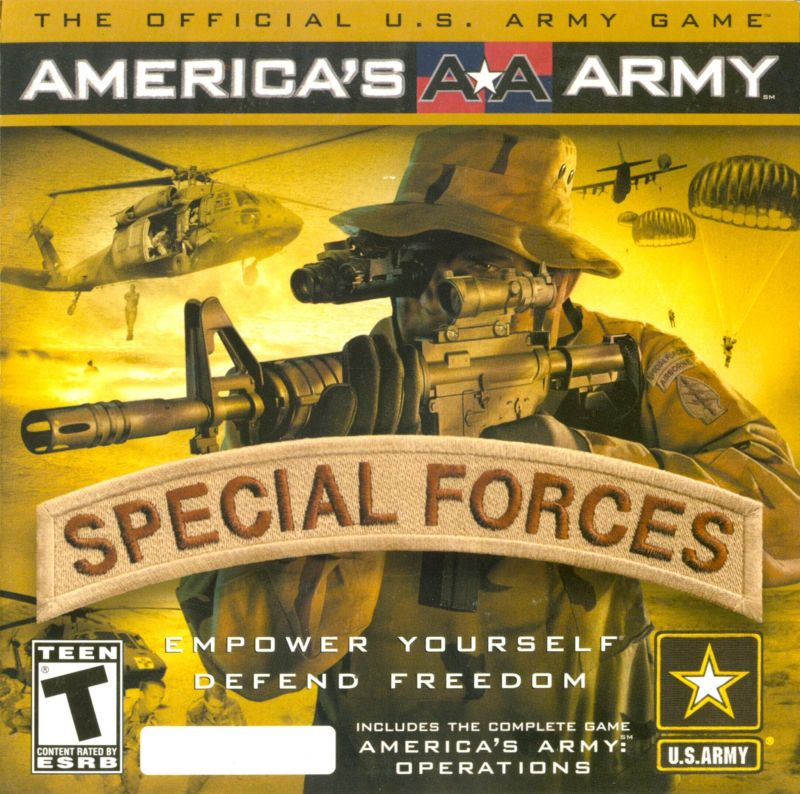
\includegraphics[scale=1]{americasarmy.jpg}
	\end{center}
	\caption{Igra koju je razvila vojska SAD-a}
\end{figure}

\newpage

\section{Nasilje u video igrama}
\label{sec:nasilje}
Neke video igre, poput {\em Grand Theft Auto (GTA)}, su ozloglašene po tome što 
nagrađuju rasnu, seksualnu, nacionalističku diskriminaciju i divljačko ponašanje. Postoje 
značajne psihološke studije o negativnom uticaju dužeg igranja ovakvih igara, koje tvrde da utiče na porast
agresivnih misli. 

Postoji Odbor za ocenjivanje softvera za zabavu {\em ESRB (Entertainment Software Rating Board)} koji kategoriše
video igre na osnovu sadržaja u njima. Kategorije koje se uzimaju o obzir su upotreba droga i alkohola, seksualni sadžaj,
količina nasilja itd. Čini se da se većina radova na etici video igara fokusira na potencijal za
jačanje ovih specifičnih ponašanja u stvarnom životu. Primer nakon koga je pokrenuta velika bura oko nasilnih video igara
se desio 2005. godine. Devin Moor je ukrao kola, a zatim upucao troje ljudi, od čega su dvoje bili policajci.
Nakon toga je izjavio kako ga je inspirisala igra {\em GTA}, koju je satima i danima igrao.\cite{cbs_devim_moor}

Postoji dosta različitih pogleda na nasilje u video igrama. Jedan je takav da dogadjaji koji se odvijaju
u video igri nisu relevantni pri etičkoj evaluaciji igre. {\em "Očigledno nasilni, sadistički i na drugi način kriminalni događaji koji se dešavaju u igricama ne mogu imati uzročno posledičnu vezu sa nasiljem u stvarnom svetu. Razlog je to što su svetovi i događaji video igara izmišljeni''} \cite{tavinor}. Za primer možemo uzeti {\em GTA} koji je
više puta osuđivan jer je dozvoljavao i podržavao igrače u izvršavanju krađa, napada, ubistva i raznih drugih nasilnih radnji.
Ali te radnje su izmišljene i ni na kakav način ne pokušavaju da razviju neki vid agresije kod pojedinca koji igra igru.
Na {\em GTA} i slične igre možemo gledati kao na {\em simulatore zločina}, slično kao i  {\em simulatori letenja},
koji dozvoljavaju svojim igračima da se prepuste u ponašanje koje vodi u opasnost. Razdvajajući ponašanje u igri
od stvarnog života je preduslov da pojedinac uživa u igri, ako bi se ono što se dešava u igri dešavalo i u stvarnom životu,
pojedinac ne bi uživao.

\begin{figure}[h!]
	\begin{center}
		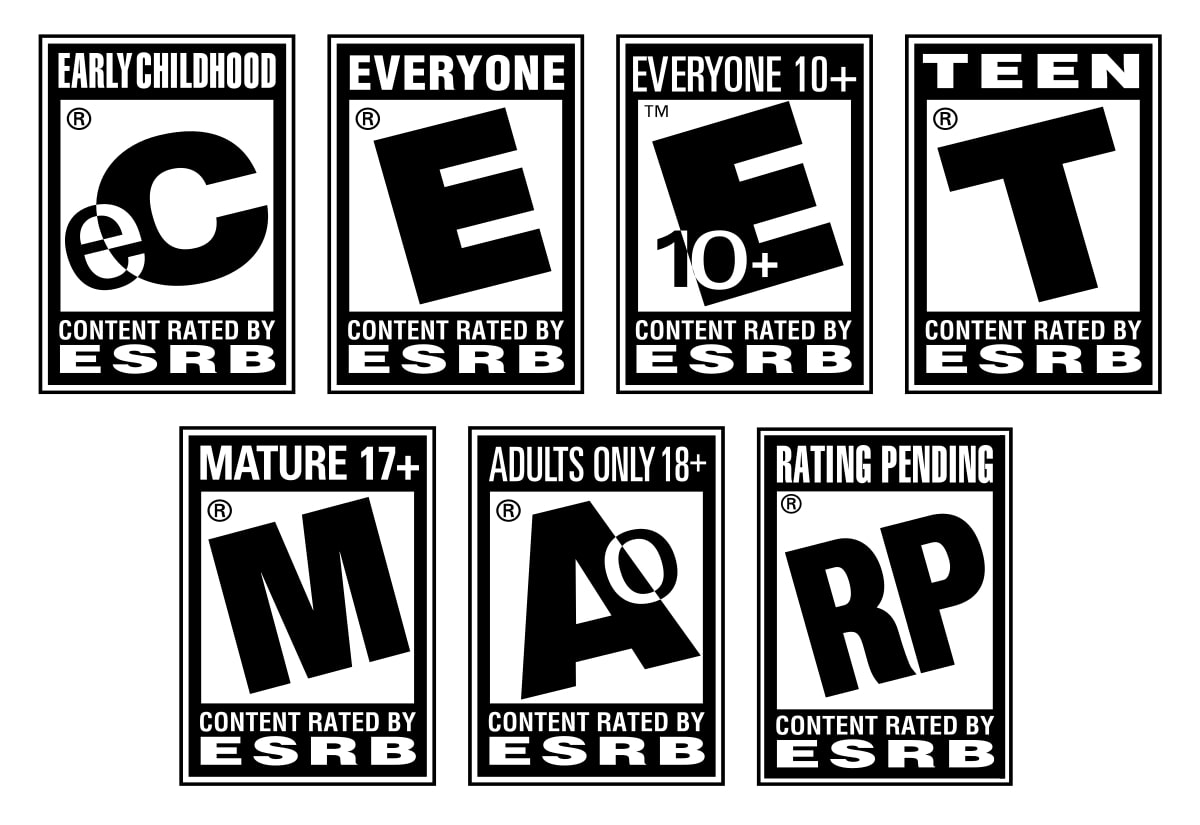
\includegraphics[scale=0.2]{ESRB.jpg}
	\end{center}
	\caption{ESRB rating}
\end{figure}

\newpage

\section{Nenasilne video igre i njihove pozitivne strane}	
\label{sec:nenasilne}
Postoje brojne video igre koje ne sadrže nasilje u sebi. Takve igre spadaju u više različitih
kategorija video igara. Postoje neke interaktivne video igre kao što su na platformi {\em Nintendo Vii} koje se
koriste u rehabilitaciji i fizikalnoj terapiji pacijenata sa moždanim udarom. Pacijenti koriste kontrolere za video igre koji simuliraju
hirurške uređaje koji im pomažu da poboljšaju reflekse.

Video igre su kategorisane prema različitom sadržaju. Ove razlike uglavnom nisu oštro definisane i često postoji
preklapanje izmedju kategorija. Jedna od kategorija višeg nivoa bi bila na {\em ozbiljne igre}. One predstavljaju aplikacije
koje bi korisnik upotrebljavao ne samo iz zabave. Primer ozbilje video igre bi bio {\em TruSim }
u kojoj se simulira eksplozija u delu grada gde je dosta ljudi, a korisnik je član hitne pomoći koji pristiže na scenu nesreće
i dobija zadatak da sortira povređene po tome koliko je hitno sanirati njihovu povredu. Edukacione igre se isto mogu svrstati u ovu kategoriju.
One su dizajnirane tako da korisnik aktivno učestvuje u njihovom sadržaju, kako bi naučio različite stvari. Igre koje se igraju 
preko interneta sa više korisnika se takođe mogu koristiti za svrhe edukacije, učenja novih veština i zabave,
ali retko ko tvrdi da ratne igre mogu da se koriste za edukaciju, osim ako možda uzmemo primer narednika iz Iraka.

Ono što je zanimljivo je činjenica da mnogi koji tvrde da nasilne video igre nemaju uticaja na čoveka isto tvrde
da edukacione igre imaju i da su veoma bitne i korisne u učenju. Reakcije na nasilje u video igrama se razlikuje
od države do države. Neke cenzurišu igre tako što neprikladan sadržaj cenzurišu, skrivanjem ili menjanjem tog 
sadržaja nečim prikladnijim, dok neke države potpuno zabranjuju takve igre.

Najveće dileme vezane za etiku kod video igara su bile zbog nasilja u njima. Ali to nije jedini razlog zašto se 
postavljaju etička pitanja u slučaju video igara. 

\begin{figure}[h!]
	\begin{center}
		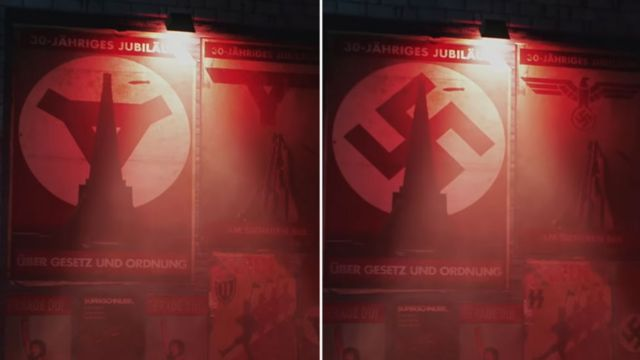
\includegraphics[scale=0.6]{wolfensteinyoungblood.jpg}
	\end{center}
	\caption{Cenzura svastike u igri Wolfenstein}
\end{figure}

\newpage
\section{Dodatni etički problemi i pristup njihovom rešavanju}
\label{sec:etika}
\subsection{Nenasilni etički problemi}
Mnogi tvrde da su video igre uzrok mnogih problema u društvu i kod pojedinaca. Neki primeri su: narušavanje zdravlja pojedinca,
rizik od zavisnosti i smanjeni akademski uspesi, koji su česti kod dece i mlađih ljudi.

Podaci o zavisnosti ili kako bi se moglo nazvati {\em entuzijazam za igru} ukazuju na ogromnu količinu vremena koju pojedinci
provedu igrajući igru. Jedan šokantan primer toga je statistika za igru {\em World of Warcraft}. Istraživanje je
pokazalo da je u jednom trenutku, 15\% ljudi koje je igralo igricu u periodu od 8 meseci, čak 2 meseca 
potrošilo igrajući igru.

Jedno vreme su se spominjali i rodni problemi sa video igrama. Gde se tvrdilo da je dečacima
ugodnije da upotrebljavaju video igre za učenje od devojaka, zbog čega one mogu da budu u zaostatku u odnosu ma dečake. 
Postoji i dosta problema sa stereotipima, na primeru igre {\em GTA}, gde su Irci predstavljeni kao pijanice, 
Rusi i Afroamerikanci kao kriminalci.

\subsection{Pristup rešavanju problema}
Mnogi razvijaoci video igara se suočavaju sa ovim problemima. Postoje različiti načini na koje oni pokušavaju da
ih reše ili zaobidju. Jedan takav je da razvijaju igre koje imaju za cilj da uče korisnika etičkim principima.
Primer takve igrice je {\em True Crime: New York City}, u kojoj igrač ima ulogu policajca. U igri je igrač kažnjen
ako uradi nešto loše a nagradjen ako uradi nešto dobro što je korisno društvu.

Dolazi se do mogućeg zaključka da možda treba uvesti neki skup pravila koji se treba poštovati pri razvijanju
video igara. Osnovni principi po kojima bi se razvijaoci igara mogli voditi bi bili:
\begin{itemize}
\item To što mogu da odluče kakve akcije su moguće u igri
\item Mogu da odluče kakve će biti posledice u igri po igrača za njegove različite akcije
\item Razvijaoci mogu da sugerišu kako treba postupati u igri na osnovu tekstova i simbola ili tako 
što će nagraditi ili kazniti igrača.
\end{itemize}  
Razvijaoci odlučuju šta su sve moguće akcije u igri i šta je njihovo značenje, što stvara dosta mogućih akcija za igrača,
te akcije mogu biti dobre, loše ili čak i nešto izmedju. Može se igra razviti tako da jedine akcije koje igrač može
da preduzme budu one koje su etički ispravne. Ali ono sa čime se mnogi slažu je to da je bolje da postoje igre kao
što je {\em True Crime: New York City} u kojima za svaku akciju, bilo to dobru ili lošu postoje posledice na osnovu 
kojih igrač može učiti.

Međutim teško je definisati u potpunosti koje su akcije dobre a koje loše, a i ako se desi nešto loše što u igri
nije pod našom kontrolom, da li tada treba predstaviti to korisniku onako kako stvarno jeste. Primer je ako se 
desi neka nesreća, da li treba staviti krv ili ne kako igrač ne bi video nešto tako. Igrač ipak i na osnovu takvih 
scena treba da donosi neke odluke u igri. Naravno moramo uzeti u obzir to da, iako razvijaoci imaju kontrolu nad
tim šta će biti sadržaj igre koju razvijaju, tu igru neko naručuje i oni moraju da ispune zahteve koje su dobili od
naručilaca softvera (igre). Ono što još treba razmatrati kada se uzme u obzir ograničavanje razvijaoca i postavljanje pravila
je to što im se time ukida njihova umetnička sloboda, a i to što postoji previše razvijaoca igara, čak i ljudi koji samostalno prave video igre
(postoje i fakultetski kursevi) što komplikuje mogućnost uvodjenja ograničenja.

Ono što je sigurno je da razvijaoci moraju biti svesni toga da video igre mogu imati uticaj na društvo, bio to
dobar ili čak loš. I moraju da razmotre kakve potencijalne ili očekivane pozitivne ili negativne efekte mogu da
imaju na pojedinca ili društvo.
\newpage

\section{Zaključak}
\label{sec:zakljucak}

Danas video igre igraju veliku ulogu u društvu. Široko su rasprostranjene na svim mestima. Svako, pa čak i deca
imaju mobilne telefone na kojima postoje video igre kao i na računarima, konzolama itd. Vidjamo ih po kladionicama, ali i u školama gde se koriste za učenje.
Imaju veliki uticaj na društvo, dobar ili loš, to se mora prihvatiti.

Sloboda pri razvijanju igara mora da postoji, to je ono što je i stvorilo tu industriju u ono što jeste. Iz te slobode
smo i dobili sve dobre strane video igara, ali moraju postojati i ograničenja kakve video igre stižu do korisnika, zato što
u zavisnosti od pojedinca mogu da utiču na loš način.

\newpage

\addcontentsline{toc}{section}{Literatura}
\appendix

\iffalse
\bibliography{reference} 
\bibliographystyle{plain}
\fi

\begin{thebibliography}{6}

\bibitem{washingtonpost} \href{https://www.washingtonpost.com/archive/politics/2006/02/14/virtual-reality-prepares-soldiers-for-real-war-span-classbankheadyoung-warriors-say-video-shooter-games-helped-hone-their-skillsspan/15996806-3a4d-4374-b066-38c5f5c35659/}{The Washington Post}
\bibitem{wikipedia_american_army} \href{https://en.wikipedia.org/wiki/America%27s_Army#Controversy}{Wikipedia}
\bibitem{cbs_devim_moor} \href{https://www.cbsnews.com/news/can-a-video-game-lead-to-murder-04-03-2005/}{CBS News}
\bibitem{tavinor} \href{https://www.ida.liu.se/~TDDI82/etik/Towards_an_Ethics_of_Video_Gaming.pdf}{Tavinor, G (2007), Towards an Ethics of Video Gaming, FuturePlay}
\bibitem{donald} \href{https://www.researchgate.net/publication/220198908_The_ethics_of_video_games_Mayhem_death_and_the_training_of_the_next_generation}{The ethics of video games: Mayhem, death, and the training of the next generation}
\bibitem{behaviour} \href{https://www.researchgate.net/publication/11792416_Effects_of_Violent_Video_Games_on_Aggressive_Behavior_Aggressive_Cognition_Aggressive_Affect_Physiological_Arousal_and_Prosocial_Behavior_A_Meta-Analytic_Review_of_the_Scientific_Literature}{Effects of Violent Video Games on Aggressive Behavior, Aggressive Cognition, Aggressive Affect, Physiological Arousal, and Prosocial Behavior: A Meta-Analytic Review of the Scientific Literature}

\end{thebibliography}

\end{document}
}
